\documentclass[final,t]{beamer}
\setbeamersize{text margin left = 25pt, text margin right = -5pt}

\usepackage{graphicx}

\usepackage{resizegather}

% poster template
% \usepackage[orientation=landscape,size=a0,scale=1.4,debug]{beamerposter}
\usepackage[orientation=landscape,size=a0,scale=1.3,debug]{beamerposter}
% \usepackage[orientation=landscape,size=custom,width=160,height=100,scale=1.8,debug]{beamerposter}
% \usepackage[ruled, vlined]{algorithm2e}
\usetheme{zurichposter}
% \usefonttheme{default}
% \usefonttheme[onlymath]{serif}

% references backend=biber, style=alphabetic, citestyle=authoryear, ,hyperref=auto
\usepackage[backend=biber,bibstyle=authoryear,citestyle=authoryear-comp]{biblatex}
\bibliography{./bibliography}

% private packages
\usepackage{color}
\usepackage{hyperref}       % hyperlinks
\usepackage{url}            % simple URL typesetting
\usepackage{booktabs}       % professional-quality tables
\usepackage{nicefrac}       % compact symbols for 1/2, etc.
\usepackage{microtype}
%\usepackage{amssymb}
\usepackage{amsmath}
%\usepackage{amsthm}
%\usepackage{amsfonts}
\usepackage{algorithm, algpseudocode}%,algorithmic}
%\usepackage[square,numbers]{natbib}
%\usepackage{natbib}
\usepackage{wrapfig}
\usepackage{subcaption}
% \usepackage{bibentry}
% \bibliography{../bibfile}
\usepackage{listings}
\lstdefinestyle{customc}{
  %belowcaptionskip=1\baselineskip,
  breaklines=true,
  language=C,
  showstringspaces=false,
  basicstyle=\footnotesize\ttfamily,
  keywordstyle=\bfseries\color{black!40!black},
  identifierstyle=\color{black}
}

\lstset{style=customc}
\usepackage{xcolor}

\floatname{algorithm}{Algorithm}
\renewcommand{\algorithmicrequire}{\textbf{Input:}}
\renewcommand{\algorithmicensure}{\textbf{return}}
\renewcommand{\algorithmicfunction}{\textbf{def}}
\algtext*{EndFunction}

\definecolor{vectorpink}{HTML}{E40086}


% -------------------- Math macros -----------------------------
%\newcommand{\norm}[1]{||#1||}
\newcommand{\etal}{\textit{et al}.}
%\newcommand{\TODO}[1]{{\color{red}TODO: #1}}
%\newcommand{\NOTE}[1]{{\color{blue}NOTE: #1}}
% \newtheorem{theorem}{Theorem}
\newtheorem*{theorem*}{Theorem}
\newcommand{\tr}{\textnormal{tr}}
\newcommand\E{\mathbb{E}}
\newcommand\R{\mathbb{R}}
%\newcommand{\B}{\mathbb{B}}
%\newcommand{\A}{\mathbb{A}}
% overwrite epsilon as varepsilon
\renewcommand{\epsilon}{\varepsilon}
%\newcommand*{\matr}[1]{\mathbfit{#1}}
\newcommand*{\tran}{^{\mkern-1.5mu\mathsf{T}}}
%\newcommand*{\conj}[1]{\overline{#1}}
%\newcommand*{\hermconj}{^{\mathsf{H}}}

\newcommand{\vx}{\mathbf{x}}
\newcommand{\vepsilon}{\mathbf{\epsilon}}
\newcommand{\vtheta}{\mathbf{\theta}}%
\newcommand{\vpsi}{{\bm{\psi}}}
\newcommand{\vpi}{{\bm{\pi}}}
\newcommand{\vphi}{{\bm{\phi}}}
\newcommand{\vz}{\mathbf{z}}
\newcommand{\vX}{\mathbf{X}}
\newcommand{\vw}{\mathbf{w}}
\newcommand{\vv}{\mathbf{v}}
\newcommand{\vr}{\mathbf{r}}
\newcommand{\vh}{\mathbf{h}}
\newcommand{\vg}{\mathbf{g}}
\newcommand{\vI}{\mathbf{I}}
\newcommand{\vzero}{{\bf{0}}}
\newcommand{\ones}[1]{\mat{1}_{#1}}
\newcommand{\eye}[1]{\mat{E}_{#1}}
\newcommand{\tra}{^{\mathsf{T}}}
\newcommand{\vect}[1]{{\bf{#1}}}
\newcommand{\mat}[1]{\mathbf{#1}}
\newcommand{\pderiv}[2]{\frac{\partial #1}{\partial #2}}
\newcommand{\npderiv}[2]{\nicefrac{\partial #1}{\partial #2}}
\newcommand{\argmin}{\operatornamewithlimits{argmin}}
\newcommand{\argmax}{\operatornamewithlimits{argmax}}
\newcommand{\expect}{\mathbb{E}}
\newcommand{\expectargs}[2]{\mathbb{E}_{#1} \left[ {#2} \right]}
\newcommand{\var}{\mathbb{V}}
\newcommand{\varL}{\mathcal{L}}
\def\iid{i.i.d.\ }
\def\simiid{\overset{\mbox{\tiny iid}}{\sim}}
\newcommand{\defeq}{\mathrel{:\mkern-0.25mu=}}
\newcommand{\Normal}{\mathcal{N}}
\newcommand{\Nt}[3]{\mathcal{N}\!\left(#1 \middle| #2,#3\right)}
\newcommand{\N}[2]{\mathcal{N}\!\left(#1,#2\right)}
\DeclareMathOperator{\KLop}{KL}
\newcommand{\KL}[2]{\KLop \left(#1 \middle \| #2 \right)}
\newcommand{\tunderbrace}[1]{\underbrace{\textstyle #1}}

\newcommand{\norm}[2][]{#1\lVert #2 #1\rVert}

%%%%%%%%%%%% Vectors %%%%%%%%%%%%%%
\def\ve#1{\mathchoice{\mbox{\boldmath$\displaystyle\bf#1$}}
{\mbox{\boldmath$\textstyle\bf#1$}}
{\mbox{\boldmath$\scriptstyle\bf#1$}}
{\mbox{\boldmath$\scriptscriptstyle\bf#1$}}}

%%%%%%%%%% Bold face letters  %%%%%%%%%%%%%
\newcommand{\rx}{{\ve r}}
\renewcommand{\u}{{\ve u}}
\newcommand{\x}{{\ve x}}
\newcommand{\w}{{\ve w}}
\newcommand{\A}{\textrm{A}}
\newcommand{\B}{\textrm{B}}

% -------------------- Define notation here --------------------

\newcommand{\latent}{\vz}
\newcommand{\hidden}{\vh}
\newcommand{\obs}{\vx}
\newcommand{\sol}{\vz}  % Solution to ODE (normally x or y}
\newcommand{\obsdim}{D_x}
\newcommand{\latentdim}{D}
\newcommand{\solvefunc}{\text{ODESolve}}
\newcommand{\tstart}{{t_\text{0}}}
\newcommand{\tend}{{t_\text{1}}}
\newcommand{\lograte}{\lambda}%\text{lograte}}
\newcommand{\method}{Latent ODE}
\newcommand{\cnfx}{\sol}


% document properties
\title{Improving PAC-Bayes bounds for neural nets}
\author{\Large Anirbit Mukherjee$^{*1}$, Pushpendre Rastogi$^{*2}$, Dan Roy$^{**}$, Jun Yang$^{**}$}
\institute{$^{*1}$ Applied Mathematics and Statistics, $^{*2}$ Computer Science, Johns Hopkins University \\$^{**}$ Statistical Sciences, Vector Institute For Artificial Intelligence, University of Toronto}


\begin{document}

\begin{frame}[containsverbatim]

\begin{columns}[t]

%-------------------------------------------------------------                          
%COLUMN 1
% ------------------------------------------------------------

\begin{column}{.32\linewidth}
    \vspace{-18mm}
    
    \begin{exampleblock}{Introduction}
    Recent works like \cite{dziugaite2017computing} and \cite{zhou2018non} have shown that one can obtain non-vacuous ``computational" PAC-Bayesian bounds on the risk of neural nets. In this work we improve on existing theoretical PAC-Bayesian risk bounds by using data-dependent priors sensitive to the geometrical properties of training and by considering carefully chosen clusters of multiple nets in tandem.  
    
    % These experiments strongly motivate the current work to search for stronger theoretical basis towards explaining the power of PAC-Bayesian risk bounds in explaining the generalization ability of neural nets. Previous PAC-Bayes bounds (and us too) have used data dependent priors on the geometric mean of the spectral norms of the layer matrices to try to track the first parameter above. In this work we also propose a mechanism of choosing the finite set priors in such a way that can also track the angular deflection in a data-dependent way. 

    % {\it Secondly,} we go further to show how in the PAC-Bayesian framework one can leverage more out of the angle parameter by simultaneously training a clusters of nets that is by obtaining in tandem a finite set of classifiers/neural functions on the chosen architecture by simultaneously training multiple instances initialized at different by closeby weight vectors. Because of this use of clusters, compared to previous bounds our dependency on the distance from initialization is also more intricate and we are able to get more sensitive to the average case behaviour. Thus we build into the theory more data-dependent (and hence tunable) parameters which help us further improve over existing bounds. And to incorporate the effect of the cluster we need to prove new noise resilience theorems for neural nets. 
    \end{exampleblock}
    
    % \begin{exampleblock}{TO DO}
    % Hello! 
    % \end{exampleblock}


    \begin{exampleblock}{Notation}
    All losses considered are multi-class margin losses. Training data-sets (denoted as $S$) will be assumed to be of size $m$ and contained in a ball of radius $B$, centered at the origin in $\R^n$.
    Define $f_{\A}: \R^n \to \R^k$ to be a depth-$d$ neural-network with maximum width $h$, whose $\ell^\text{th}$ layer has weight matrix $\A_\ell$. The first $d-1$ layers of $f_{\A}$ use the \textsc{Relu} non-linear activation. $\A$ is the vector of parameters formed by concatenating vectorized layer matrices, i.e. $\A$ denotes the vector $[\mathrm{vec}(\A_1); \ldots; \mathrm{vec}(\A_d)]$ whose each coordinate is a distinct trainable weight in the net.
    %Let ${\cal N}_{(\A,\sigma^2)}$ denote the isotropic multivariate Gaussian probability distribution with mean $\A$ and variance $\sigma^2 \mathbf{I}$
    \newline \\
    Define $\beta(\A) = \big ( \prod\nolimits_{\ell=1}\nolimits^d \norm{A_\ell}_2 \big )^{1/d}$. We will omit the argument $\A$ whenever the neural-network under consideration is clear from the context. {\it Clearly $\beta^d$ upperbounds the Lipschitz-constant for $f_{\A}$.}
    \newline \\ 
    Let $\{ {\A}_i \in \R^{\dim(\A)} \mid  i=1,..,k_1 \}$ denote a set of $k_1 \geq 2$ neural net weight vectors on the underlying architecture of $f_{\A}$. Let $\{p_i \mid i=1, \ldots, k_1\}$ be a set of non-zero scalars s.t $\sum_i p_i = 1$. Define $\beta_i := \beta(\A_i)$.  
   \end{exampleblock}
   
   \begin{exampleblock}{Controlled output perturbation with a mixture of Gaussians sampling for the weights}
    \begin{theorem}[{\bf 1}] 
    Suppose the following condition holds for some $\epsilon >0$, 
    %\vspace{-2mm} 
    \[ \forall i {\in} \{1\ldots k_1\}, \x {\in} S\  \norm{f_{\A_i}(\x) {-} f_{\A}(\x)} \leq \epsilon \norm{f_{\A}(\x)} \]
    %\vspace{-3mm} 
    Then for every $\gamma > \epsilon \max_{\x \in S} \norm{f_{\A}(\x)}$, we have,
    \begin{align} 
    \nonumber \mathbb{P}_{A' \sim \text{MG(posterior)}}
    &{\Big[} \max_{\x \in S} \norm{f_{A'}(\x) {-} f_A(\x)} {>} 2 \gamma  {\Big]}
    \leq \delta
    \end{align}
    ~\\ 
    Where $\text{MG(posterior)}(\w) = \sum_i p_i \mathcal{N}_{(\A_i, \sigma^2)}(\w)$ 
    ~\\ and $\sigma \le \frac{1}{\sqrt{2h \log \left ( \frac{2dhk_1}{\delta} \right )}}  \min_{1 \le i \le k_1} \min \left \{ \frac{ \beta_i }{d} , \frac{\gamma}{k_1 edB p_i \beta_i ^{d-1}}  \right \}$. \qed 
    \end{theorem} 
    \begin{center}
        {\it \color{violet} Now we will use this above noise resilience theorem about nets to get finer data-dependent PAC-Bayesian risk bounds on neural nets.}
    \end{center}
    \end{exampleblock}
    
    \begin{exampleblock}{Defining ``Nice'' training dataset}
    We call a training dataset $S$ as $(\epsilon,\gamma)-$nice w.r.t neural weight vectors $\A$ and $\{\A_i\}_{i=1}^{k_1}$ if it satisfies the following two conditions, 
    \begin{enumerate}
    \item $\max_{\x \in S} \norm{f_{\A_i}(\x) - f_{\A}(\x)} \leq \epsilon \norm{f_{\A}(\x)}, \forall 1 {\le} i {\le} k_1$
    \item $\gamma > \epsilon \max_{\x \in S} \norm{f_{\A}(\x)}$
    \end{enumerate}
    \end{exampleblock}
\end{column}


%-------------------------------------------------------------------------         
%COLUMN 2
% ------------------------------------------------------------------------


\begin{column}{.32\linewidth}
\vspace{-18mm}







\begin{exampleblock}{A two dimensional grid of priors}
  Let $\Lambda = \{1,\ldots,314\}$ and choose a regularization parameter $d_{\min} >0$. For each $\lambda \in \Lambda$ we choose $k_1$ distinct neural net weights $\{ \B_{\lambda,j} \}_{j=1}^{k_1}$ within a conical half-angle of $0.01\lambda$ around the initial neural weight $\B$. 
\newline \\ 
For each $\lambda$, we construct a grid $\mathcal{B}_\lambda$, (call it  the ``beta-grid"), containing at most $K_1$ points in a fixed compact interval in $\R$. ({\it Neither the grid points nor the interval depend on $\lambda$ but they do depend on the parameters $B,d,h,\gamma,m,\delta$ and $d_{\min}$}). 
  \newline \\ 
  For each $\lambda \in \Lambda$ and $\tilde{\sigma} \in \mathcal{B}_\lambda$ we consider the following mixture of Gaussians $\frac{1}{k_1}\sum_{j=1}^{k_1}  {\cal N}_{(\B_{\lambda,j},\tilde{\sigma}^2 I)}$.  Thus we have a grid of priors of total size $K := 314K_1$.
\end{exampleblock}



\begin{exampleblock}{A new PAC-Bayesian risk bound on nets}
    \begin{theorem}[{\bf 2}]
    Suppose we train using a dataset $S$ to obtain the trained net $f_{\A}$ from an initial neural net $f_{\B}$. Let $\theta = \arccos\frac{\langle \A, \B \rangle}{\norm{\A}, \norm{\B}}$. Let $\lambda^* = \argmin_{\lambda \in \Lambda}|0.01\lambda - \theta|$.  
    \newline \\ 
    Let the neural weights $\{ \A_i\}_{i=1,\ldots,k_1}$ be obtained by training the nets $\{ f_{\B_{\lambda^*,j}} \}_{j=1,\ldots,k_1}$ on $S$ and suppose $S$ is $(\epsilon,\gamma)-$nice w.r.t $\{ \A, \A_{i=1,\ldots,k_1} \}$
    \newline \\ 
    Now for each such $i$ define $d_{i, _*} = \min_{j=1,\ldots,k_1} \norm{\A_i - \B_{\lambda^*,j}}^2$ and $\tilde{\beta}_i = \argmin_{x \in \mathcal{B}_{\lambda^*}} | x - \beta(\A_i)|$ Then it follows that for all $\epsilon >0$ and $\delta \in (0,\frac{1}{K})$, 
    %\vspace{-2mm}  
    %{\small
    \begin{align}
    \nonumber &\mathbb{P}_{S} \Bigg [ \exists\, 
    \tilde{\mu}_{\A} \text{ s.t. }, \forall i \text{ s.t. } d_{i,_*} \geq d_{\min},  \mathbb{E}_{\A + \tilde{\u} \sim \tilde{\mu}_{\A}} [ L_{0} (f_{\A + \tilde{\u}}) ] \leq \hat{L}_{\frac \gamma 2} \left (f_{\A} \right ) +\\
    &\nonumber \sqrt{\frac 1 {m-1}}\sqrt{{-\log\Big(  \frac{1}{k_1} \sum\nolimits_{j=1}\nolimits^{k_1}    \exp(- {\frac 1 {2\tilde{\sigma}_i^2}}\|\A_i - \B_{\lambda^*,j}\|^2) \Big) + \log \frac{3m}{\delta}}} \\
    &  \Bigg]\geq 1 - K\delta \label{eq:ours}
    \end{align}
    %}

    where $\tilde{\sigma}_i^2 := \frac{1}{2h \log \left ( \frac{2dh}{\delta} \right )}  \left (  \min \left \{  \frac{ \tilde{\beta}_i }{de^{\frac {1}{d-1}}} , \frac{\frac \gamma 8}{e^2dB \tilde{\beta}_i ^{d-1}}  \right \}  \right )^2$ 
    \end{theorem} 
\end{exampleblock}

\begin{exampleblock}{Some salient points about the (main) Theorem ($2$)}
\vspace{12mm} 
\begin{enumerate}
\item The distribution $\tilde{\mu}_{\A}$ is explicitly constructed such that when the noisy weights above $\A +\tilde{\u}$ are sampled from this distribution, it is ensured that $\max_{\x \in S} \norm{ f_{\A + \tilde{\u}} (\x) - f_{\A} (\x)}_\infty < \frac{\gamma}{4}$.
Also note that as defined above, $\lambda^*$ is the closest angle in the set  $\{0.01,0.02,\ldots,3.14\}$ to the angle between the initial net's weight vector $\B$ and the trained net's weight vector $\A$
\vspace{12mm} 
\item In our experiments the nets $\{ \A_i\}_{i=1,\ldots,k_1}$ were obtained by training the nets $\{ f_{\B_{\lambda^*,j}} \}_{j=1,\ldots,k_1}$ on $S$ by the same algorithm by which we obtained $f_{\A}$ from $f_{\B}$. A direction to explore further is if (maybe data-dependent) compression techniques can be used to obtain particularly good clusters of $\{B_{\lambda^*,j}\}$ from $\B$ and $\{\A_i\}$ from $\A$.
\end{enumerate}
\end{exampleblock}


\end{column}





%------------------------------------------
%Column 3
%------------------------------------------



\begin{column}{.32\linewidth}
\vspace{-18mm}

\begin{exampleblock}{Comparison with ~\cite{neyshabur2017pac} on CIFAR-10}

In the following figure we see examples of how \textsc{Our} bounds do better than \textsc{NBS} (~\cite{neyshabur2017pac}) . We plot \textsc{Our} bound for the $i^{\text{th}}$ point in the final cluster (as defined in equation \ref{eq:ours}) that achieves the lowest bound. Note the log-scale in the $y-$axis in this figure and hence the relative advantage of our bound is a significant multiplicative factor which is {\it increasing} with depth. {\it And at large widths our bound seems to essentially flatten out in its depth dependence.}
~\\~\\ 
\begin{figure}
\begin{subfigure}[b]{.45\columnwidth}
    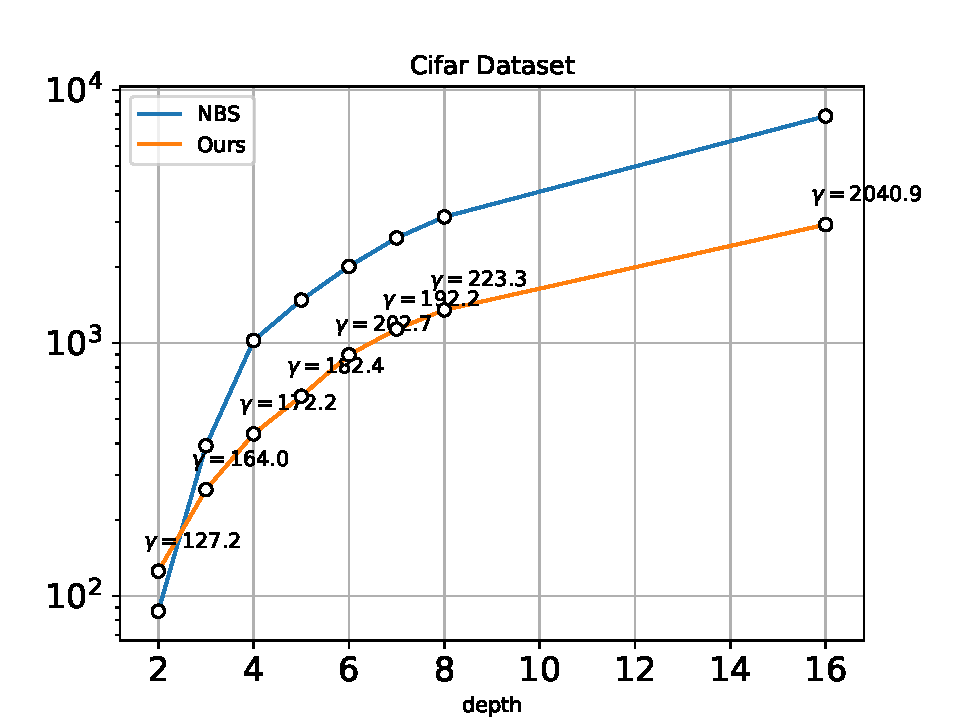
\includegraphics[trim=0 15 0 35,clip,width=\linewidth]{dcifar.pdf}
\end{subfigure}
\hfill 
\begin{subfigure}[b]{.45\columnwidth}
   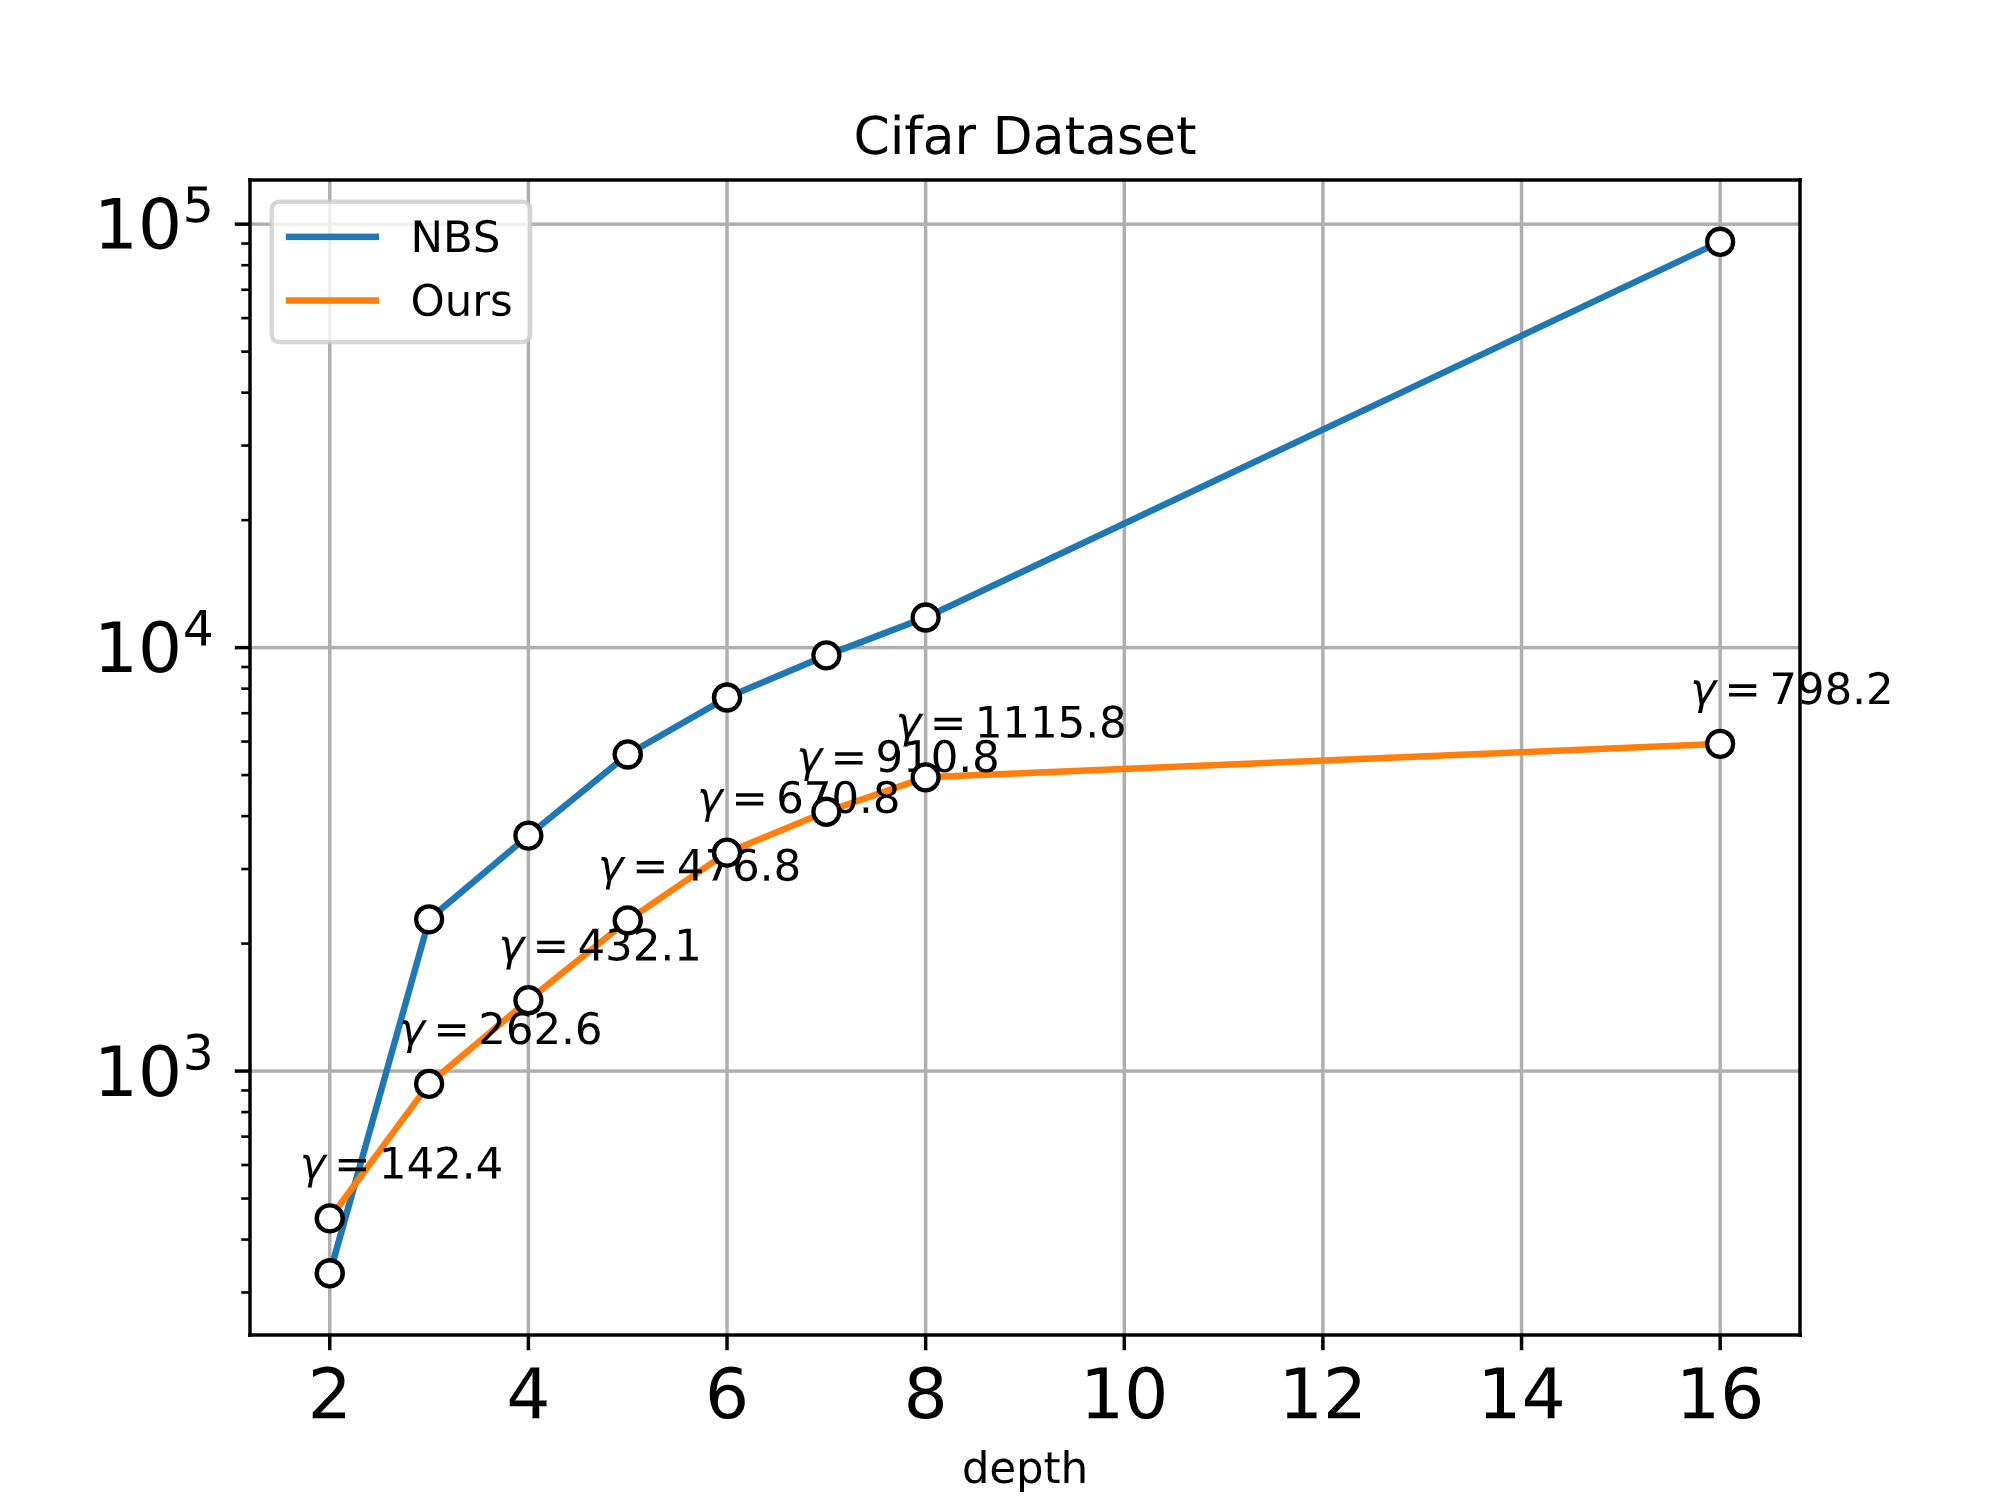
\includegraphics[trim=0 80 0 170,clip,width=\linewidth]{CIFAR_Width_400.png}
\end{subfigure}
\caption{Net width is 100 on left and 400 on the right.}
\label{fig:dcif}
\end{figure}
\end{exampleblock}


\begin{exampleblock}{Demonstration of stability of the relevant geometrical properties of training}
\vspace{2.2mm}
In the {\it \color{violet} figure to the left} we plot the initial parameter norm $\norm{\B}_2$ vs the final parameter norm $\norm{\A}_2$ for training nets of different depths at width $100$ on the CIFAR-10 dataset. Thus its demonstrated that the multiplicative factor with which the norm increases during training is fairly stable to architectural changes. 

\begin{figure}[htbp]
  \begin{subfigure}[b]{.45\textwidth}
    \centering
  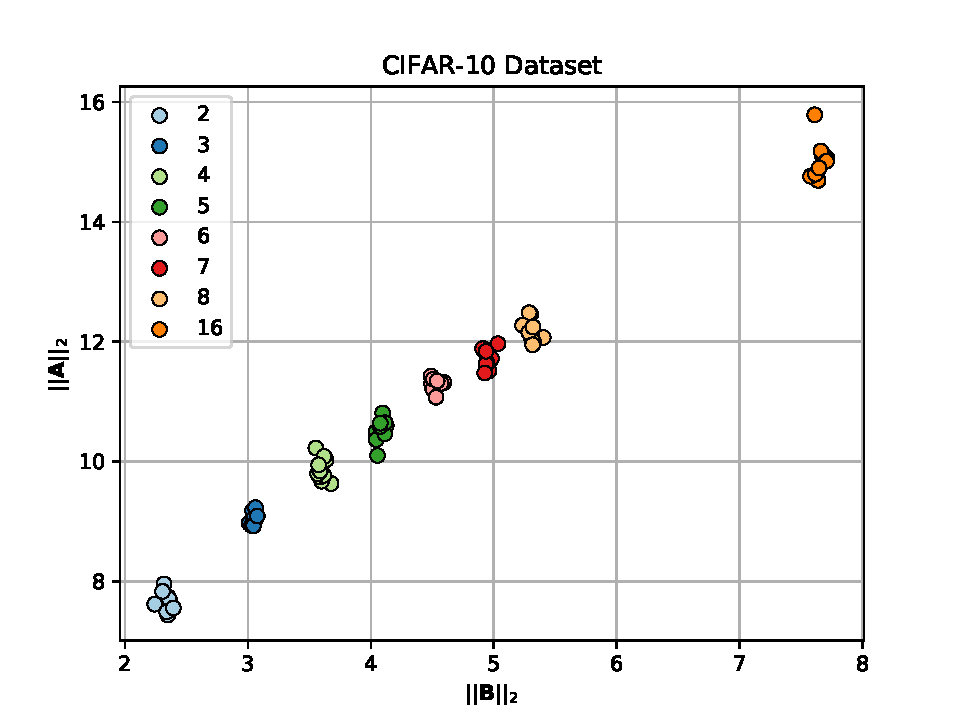
\includegraphics[width=\textwidth]{dcifstorel2norm.pdf}
  \end{subfigure}
  %\caption{Initial parameter norm $\norm{\B}_2$ vs final parameter norm $\norm{\A}_2$ with increasing depths (at width $100$) on the CIFAR-10 dataset. $10$ trials are displayed for each architecture.}
  %\label{fig:dcifstorel2norm}
  \hfill 
  \hspace{-10mm} 
  \begin{subfigure}[b]{.45\textwidth}
    \centering
  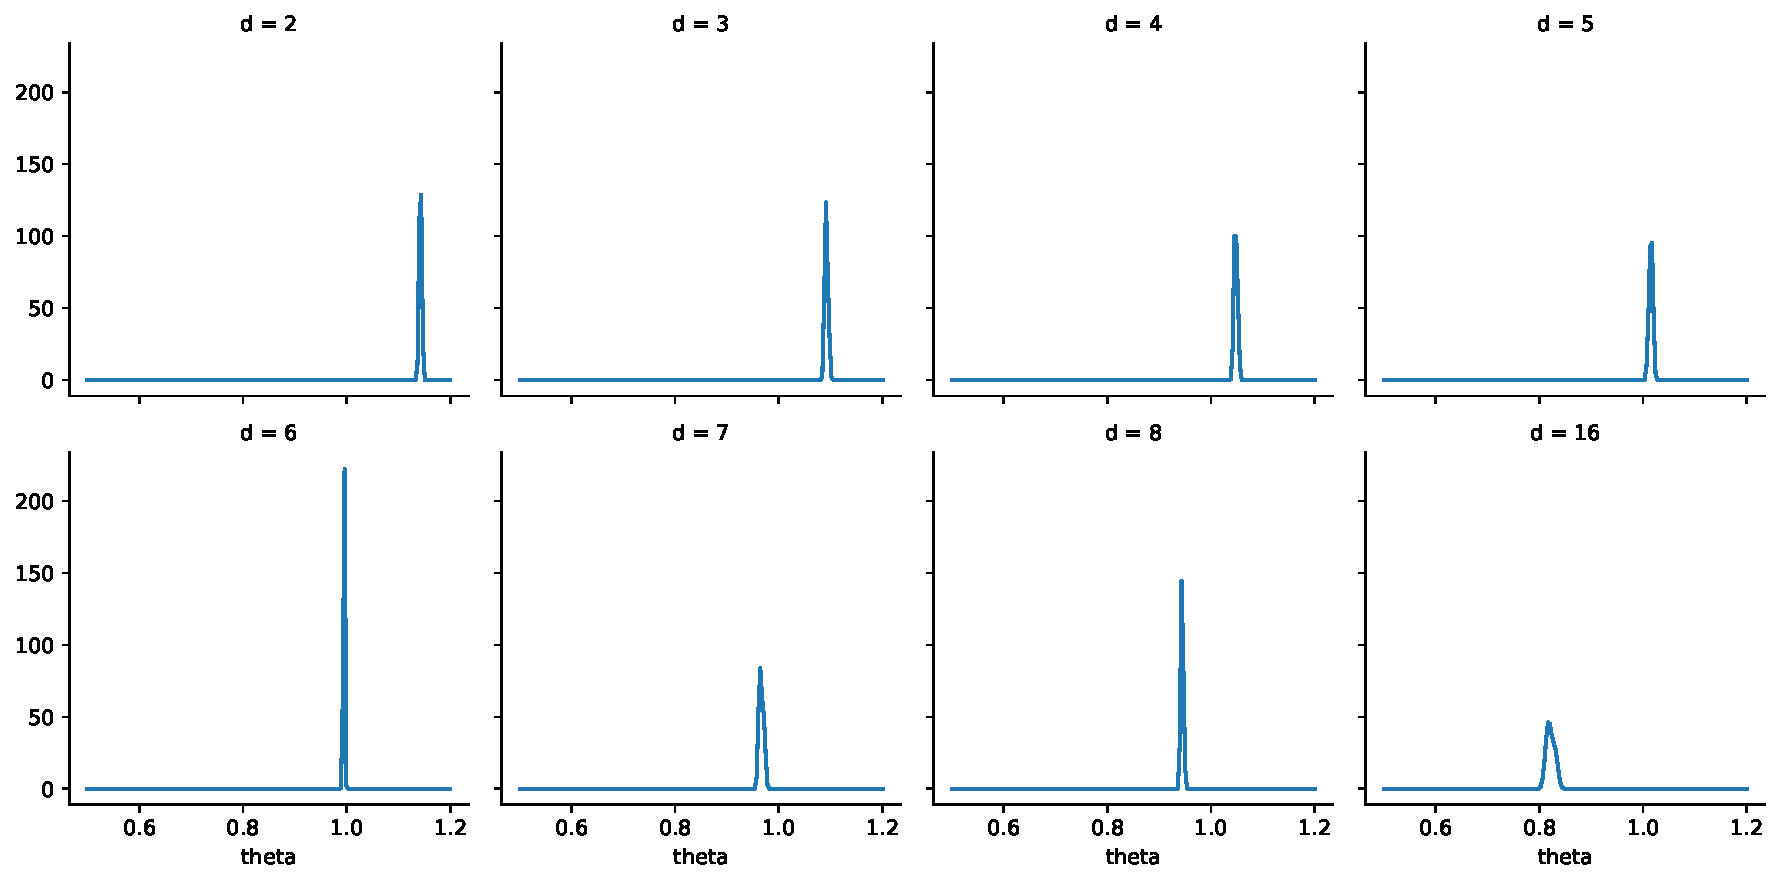
\includegraphics[width=0.95\textwidth]{dcif_kdetheta.pdf}
  %\caption{}
  %\caption{(Left) Initial parameter norm $\norm{\B}_2$ vs final parameter norm $\norm{\A}_2$ with increasing depths (at width $100$) on the CIFAR-10 dataset. $10$ trials are displayed for each architecture.  (Right) Gaussian kernel density estimate on $10$ trials of the experiment (for every depth $d$ and $100$ width) measuring the angular deviation of the weight vector under training}
  %\label{fig:dciftheta}
  \end{subfigure} 
\end{figure}

In the {\it \color{violet} figure to the right} is displayed the Gaussian kernel density estimate on $10$ trials of the experiment (at different depths and $100$ width) measuring the angular deviation of the weight vector under training. This deflection angle only decreases slightly with depth and showed negligible dependence over the widths tried. 
\vspace{2.2mm}
% \begin{figure}[htbp]
%   \centering
%   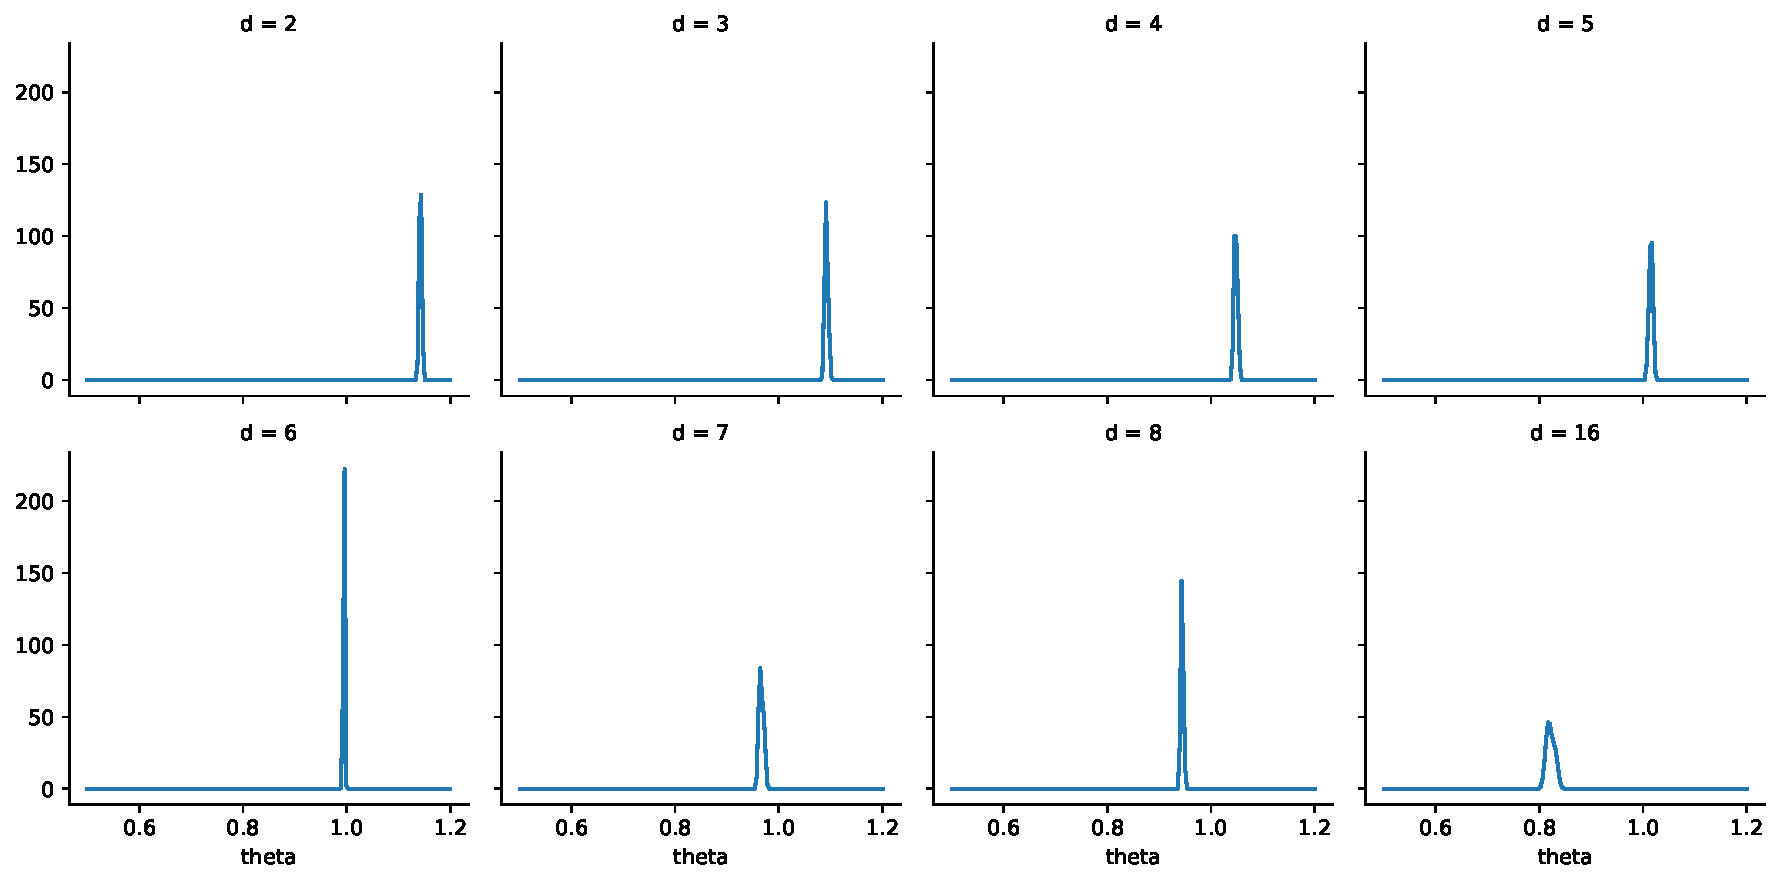
\includegraphics[width=0.5\linewidth]{dcif_kdetheta.pdf}
%   \caption{Gaussian kernel density estimate on $10$ trials of the experiment (for every depth $d$ and $100$ width) measuring the angular deviation of the weight vector under training}
%   \label{fig:dciftheta}
% \end{figure}

\end{exampleblock}


\begin{exampleblock}{References}
    %\small 
    \vspace{1mm} 
\printbibliography
\vspace{1mm} 
\end{exampleblock}

\end{column}

\end{columns}
\end{frame}

\end{document}






% \nocite{*}
% \tiny {\bibliographystyle{plainnat}}